\documentclass[11pt,a4paper]{report}
\usepackage[textwidth=37em,vmargin=30mm]{geometry}
\usepackage{calc,xunicode,amsmath,amssymb,paralist,enumitem,tabu,booktabs,datetime2,xeCJK,xeCJKfntef,listings}
\usepackage{tocloft,fancyhdr,tcolorbox,xcolor,graphicx,eso-pic,xltxtra,xelatexemoji}

\newcommand{\envyear}[0]{2025}
\newcommand{\envdatestr}[0]{2025-02-11}
\newcommand{\envfinaldir}[0]{webdb/2025/20250211/final}

\usepackage[hidelinks]{hyperref}
\hypersetup{
    colorlinks=false,
    pdfpagemode=FullScreen,
    pdftitle={Web Digest - \envdatestr}
}

\setlength{\cftbeforechapskip}{10pt}
\renewcommand{\cftchapfont}{\rmfamily\bfseries\large\raggedright}
\setlength{\cftbeforesecskip}{2pt}
\renewcommand{\cftsecfont}{\sffamily\small\raggedright}

\setdefaultleftmargin{2em}{2em}{1em}{1em}{1em}{1em}

\usepackage{xeCJK,xeCJKfntef}
\xeCJKsetup{PunctStyle=plain,RubberPunctSkip=false,CJKglue=\strut\hskip 0pt plus 0.1em minus 0.05em,CJKecglue=\strut\hskip 0.22em plus 0.2em}
\XeTeXlinebreaklocale "zh"
\XeTeXlinebreakskip = 0pt


\setmainfont{Brygada 1918}
\setromanfont{Brygada 1918}
\setsansfont{IBM Plex Sans}
\setmonofont{JetBrains Mono NL}
\setCJKmainfont{Noto Serif CJK SC}
\setCJKromanfont{Noto Serif CJK SC}
\setCJKsansfont{Noto Sans CJK SC}
\setCJKmonofont{Noto Sans CJK SC}

\setlength{\parindent}{0pt}
\setlength{\parskip}{8pt}
\linespread{1.15}

\lstset{
	basicstyle=\ttfamily\footnotesize,
	numbersep=5pt,
	backgroundcolor=\color{black!5},
	showspaces=false,
	showstringspaces=false,
	showtabs=false,
	tabsize=2,
	captionpos=b,
	breaklines=true,
	breakatwhitespace=true,
	breakautoindent=true,
	linewidth=\textwidth
}






\newcommand{\coverpic}[2]{
    % argv: itemurl, authorname
    Cover photo by #2~~(\href{#1}{#1})
}
\newcommand{\makeheader}[0]{
    \begin{titlepage}
        % \newgeometry{hmargin=15mm,tmargin=21mm,bmargin=12mm}
        \begin{center}
            
            \rmfamily\scshape
            \fontspec{BaskervilleF}
            \fontspec{Old Standard}
            \fontsize{59pt}{70pt}\selectfont
            WEB\hfill DIGEST
            
            \vfill
            % \vskip 30pt
            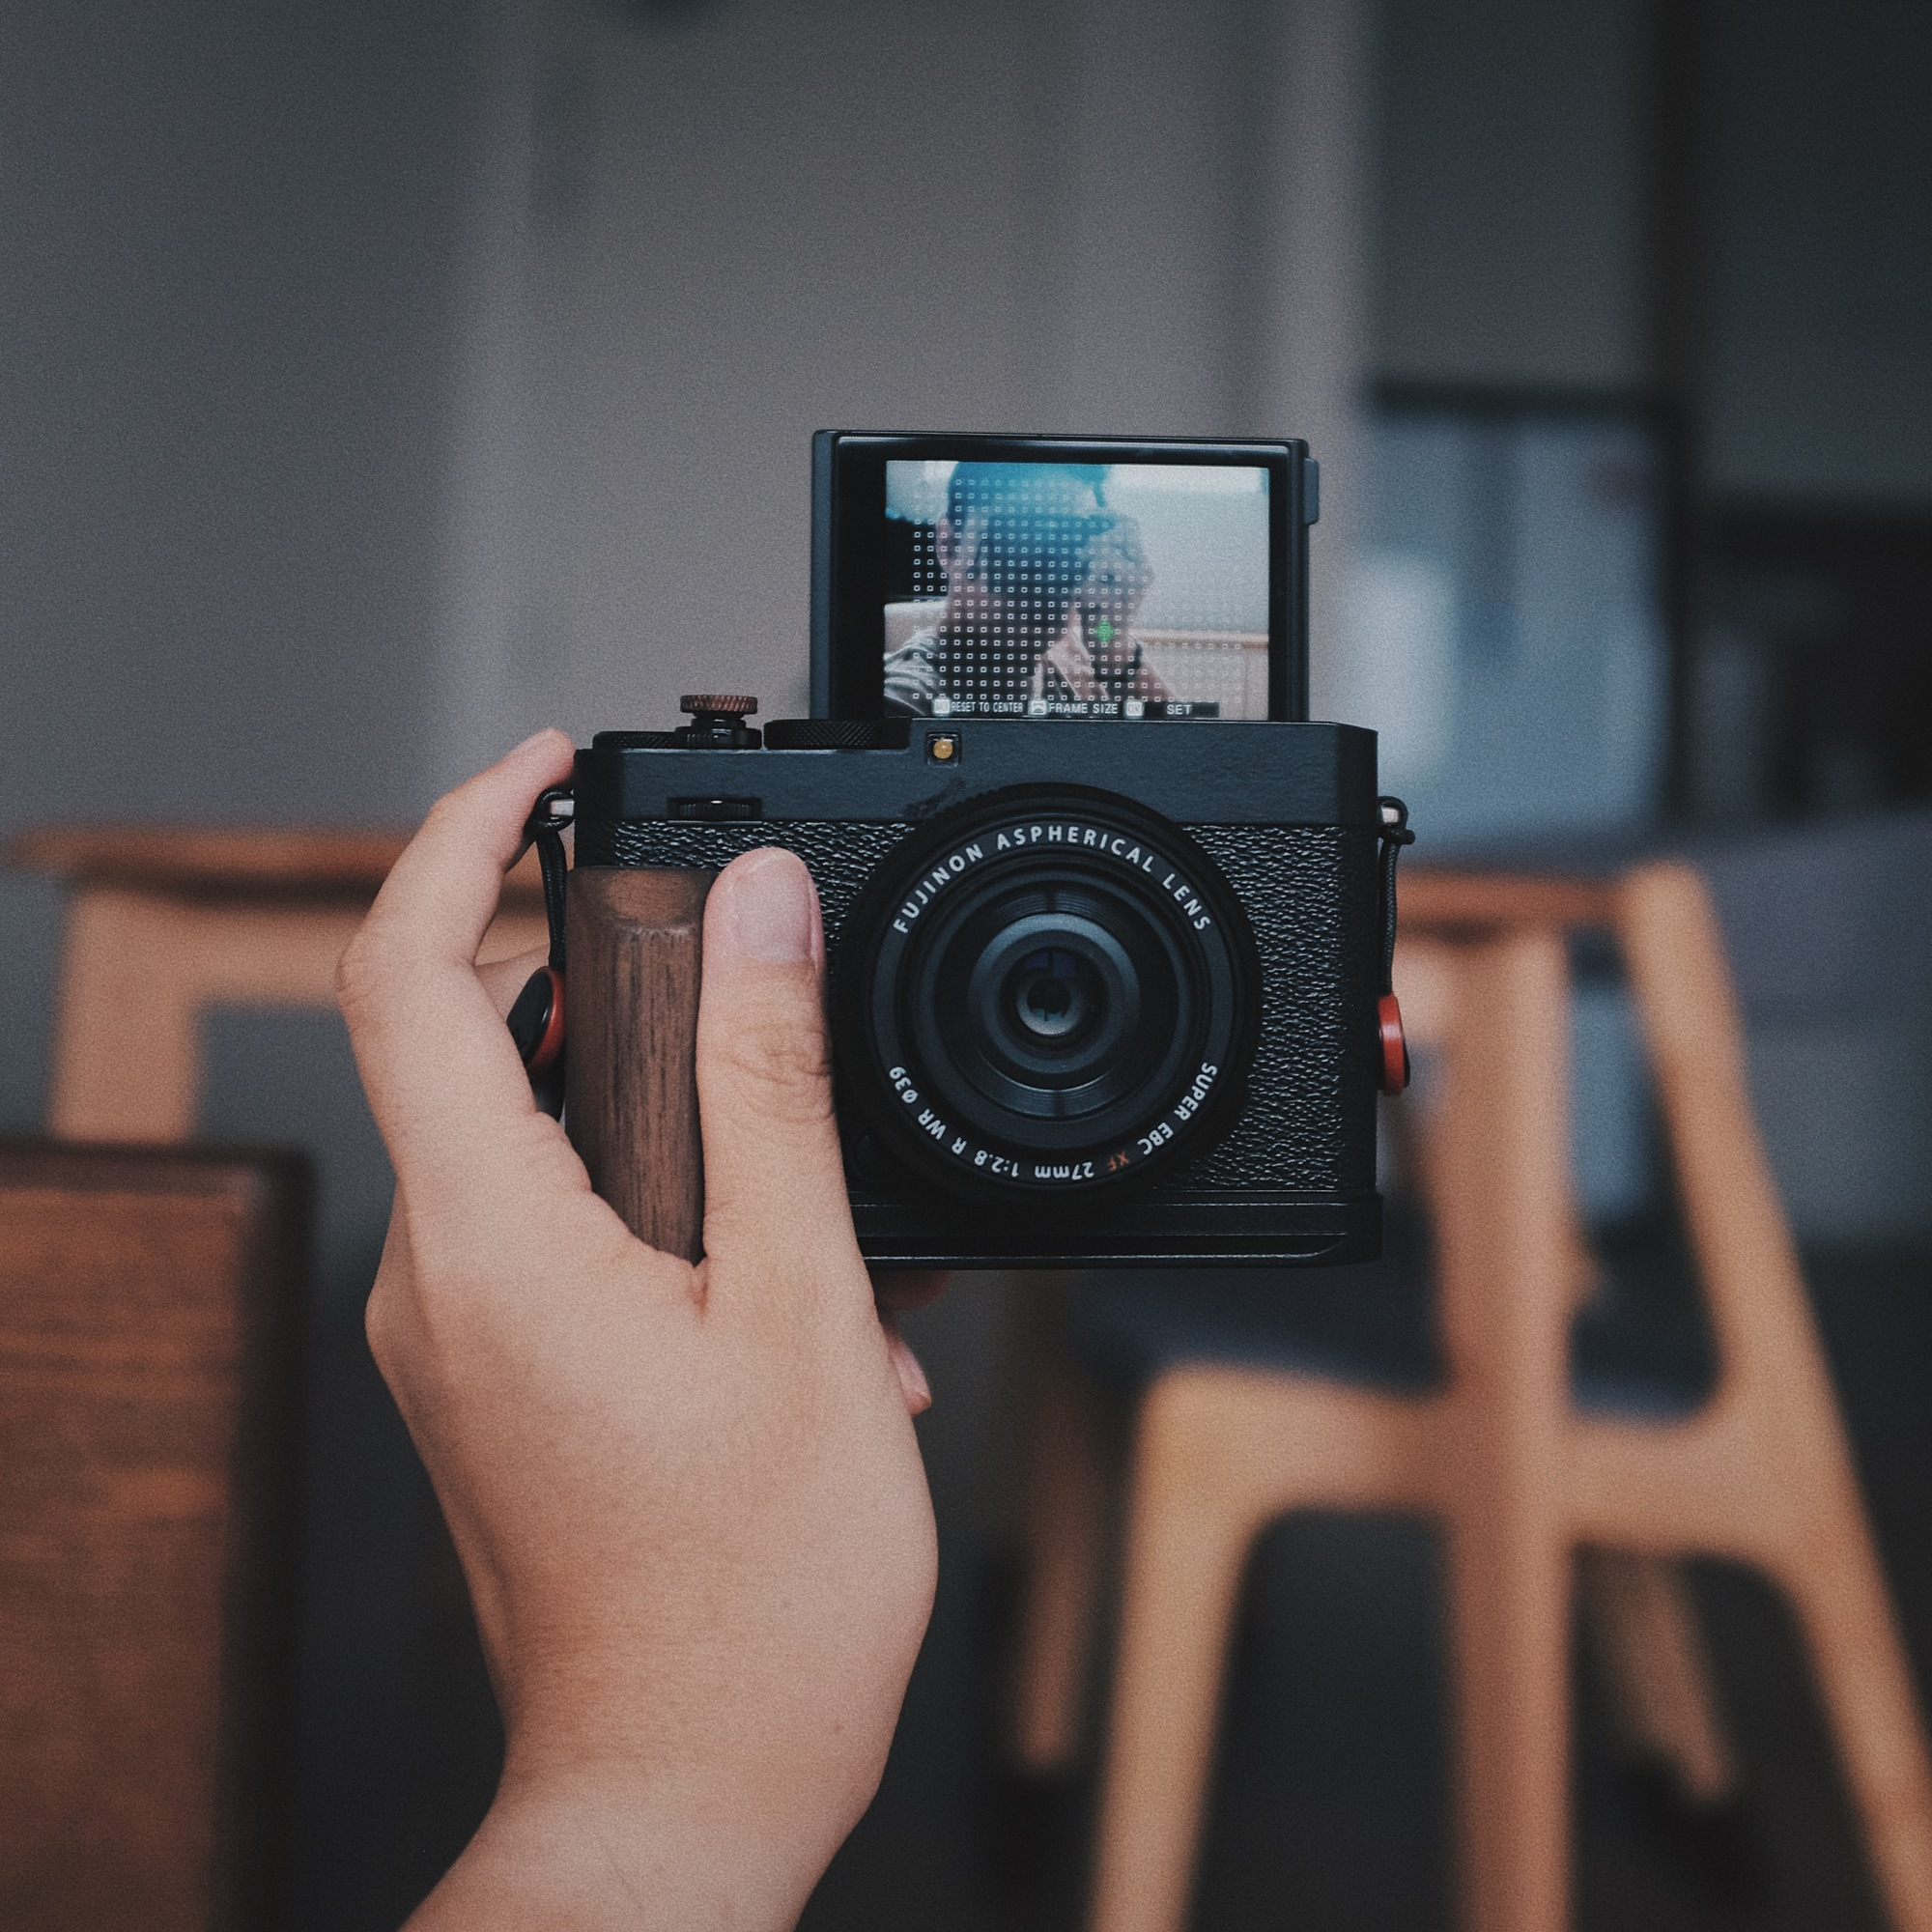
\includegraphics[width=\linewidth]{\envfinaldir/coverpic-prod.jpg}\par
            % \vskip 30pt
            \vfill

            \normalsize\rmfamily\scshape
            \copyright{} The Web Digest Project \hfill\large \envdatestr
        \end{center}
    \end{titlepage}
    % \restoregeometry
}
\newcommand{\simplehref}[1]{%
    \textcolor{blue!80!green}{\href{#1}{#1}}%
}
\renewcommand{\contentsname}{\center\Huge\sffamily\bfseries Contents\par\vskip 20pt}
\newcounter{ipartcounter}
\setcounter{ipartcounter}{0}
\newcommand{\ipart}[1]{
    % \vskip 20pt
    \clearpage
    \stepcounter{ipartcounter}
    \phantomsection
    \addcontentsline{toc}{chapter}{#1}
    % \begin{center}
    %     \Huge
    %     \sffamily\bfseries
    %     #1
    % \end{center}
    % \vskip 20pt plus 7pt
}
\newcounter{ichaptercounter}
\setcounter{ichaptercounter}{0}
\newcommand{\ichapter}[1]{
    % \vskip 20pt
    \clearpage
    \stepcounter{ichaptercounter}
    \phantomsection
    \addcontentsline{toc}{section}{\numberline{\arabic{ichaptercounter}}#1}
    \begin{center}
        \Huge
        \sffamily\bfseries
        #1
    \end{center}
    \vskip 20pt plus 7pt
}
\newcommand{\entrytitlefont}[1]{\subsection*{\raggedright\Large\sffamily\bfseries#1}}
\newcommand{\entryitemGeneric}[2]{
    % argv: title, url
    \parbox{\linewidth}{
        \entrytitlefont{#1}\par\vskip 5pt
        \footnotesize\ttfamily\mdseries
        \simplehref{#2}
    }\vskip 11pt plus 11pt minus 1pt
}
\newcommand{\entryitemGithub}[3]{
    % argv: title, url, desc
    \parbox{\linewidth}{
        \entrytitlefont{#1}\par\vskip 5pt
        \footnotesize\ttfamily\mdseries
        \simplehref{#2}\par\vskip 5pt
        \small\rmfamily\mdseries#3
    }\vskip 11pt plus 11pt minus 1pt
}
\newcommand{\entryitemAp}[3]{
    % argv: title, url, desc
    \parbox{\linewidth}{
        \entrytitlefont{#1}\par\vskip 5pt
        \footnotesize\ttfamily\mdseries
        \simplehref{#2}\par\vskip 5pt
        \small\rmfamily\mdseries#3
    }\vskip 11pt plus 11pt minus 1pt
}
\newcommand{\entryitemHackernews}[3]{
    % argv: title, hnurl, rawurl
    % \parbox{\linewidth}{
    %     \entrytitlefont{#1}\par\vskip 5pt
    %     \footnotesize\ttfamily\mdseries
    %     \simplehref{#3}\par
    %     \textcolor{black!50}{\href{#2}{#2}}
    % }\vskip 11pt plus 11pt minus 1pt
    \begin{minipage}{\linewidth}
            \entrytitlefont{#1}\par\vskip 5pt
            \footnotesize\ttfamily\mdseries
            \simplehref{#3}\par
            \textcolor{black!50}{\href{#2}{#2}}
    \end{minipage}\par\vskip 11pt plus 11pt minus 1pt
}







\begin{document}

\makeheader

\tableofcontents\clearpage




\ipart{Developers}
\ichapter{Hacker News}
\entryitemTwoLinks{Musk-led group makes \$97B bid for control of OpenAI}{https://news.ycombinator.com/item?id=43004889}{https://www.reuters.com/markets/deals/elon-musk-led-group-makes-974-billion-bid-control-openai-wsj-reports-2025-02-10/}

\entryitemTwoLinks{Kaspersky finds hardware backdoor in 5 generations of Apple Silicon (2024)}{https://news.ycombinator.com/item?id=43003230}{https://www.xstore.co.za/stuff/2024/01/kaspersky-finds-hardware-backdoor-in-5-generations-of-apple-silicon/}

\entryitemTwoLinks{1\% Equity for Founding Engineers Is BS}{https://news.ycombinator.com/item?id=43002999}{https://fetchfox.ai/a/founding-engineer-compensation}

\entryitemTwoLinks{Undergraduate shows that searches within hash tables can be much faster}{https://news.ycombinator.com/item?id=43002511}{https://www.quantamagazine.org/undergraduate-upends-a-40-year-old-data-science-conjecture-20250210/}

\entryitemTwoLinks{CAPTCHAs: 'a tracking cookie farm for profit masquerading as a security service'}{https://news.ycombinator.com/item?id=43002440}{https://www.pcgamer.com/gaming-industry/a-2023-study-concluded-captchas-are-a-tracking-cookie-farm-for-profit-masquerading-as-a-security-service-that-made-us-spend-819-billion-hours-clicking-on-traffic-lights-to-generate-nearly-usd1-trillion-for-google/}

\entryitemTwoLinks{Show HN: Open Source Security \& Compliance: Introducing Opencomply}{https://news.ycombinator.com/item?id=43001826}{https://opencomply.io}

\entryitemTwoLinks{Bank CEO: Retract your debanking piece? Me: No}{https://news.ycombinator.com/item?id=43001441}{https://www.kalzumeus.com/2025/02/10/retraction-request-denied/}

\entryitemTwoLinks{The Anthropic Economic Index}{https://news.ycombinator.com/item?id=43000529}{https://www.anthropic.com/news/the-anthropic-economic-index}

\entryitemTwoLinks{Surnames from nicknames nobody has any more}{https://news.ycombinator.com/item?id=43000316}{https://blog.plover.com/lang/etym/nickname-names.html}

\entryitemTwoLinks{Show HN: HTML visualization of a PDF file's internal structure}{https://news.ycombinator.com/item?id=43000303}{https://github.com/desgeeko/pdfsyntax/blob/main/docs/browse.md}

\entryitemTwoLinks{What about K?}{https://news.ycombinator.com/item?id=42999650}{https://xpqz.github.io/kbook/Introduction.html}

\entryitemTwoLinks{I built an open source AI tool to find my autoimmune disease}{https://news.ycombinator.com/item?id=42999632}{https://old.reddit.com/r/selfhosted/comments/1ij7s4m/how\_i\_built\_an\_open\_source\_ai\_tool\_to\_find\_my/}

\entryitemTwoLinks{Advertising Is a Cancer on Society (2019)}{https://news.ycombinator.com/item?id=42999561}{https://jacek.zlydach.pl/blog/2019-07-31-ads-as-cancer.html}

\entryitemTwoLinks{The state of Rust trying to catch up with Ada [video]}{https://news.ycombinator.com/item?id=42998061}{https://fosdem.org/2025/schedule/event/fosdem-2025-5356-the-state-of-rust-trying-to-catch-up-with-ada/}

\entryitemTwoLinks{To buy a Tesla Model 3, only to end up in hell}{https://news.ycombinator.com/item?id=42998024}{https://www.myteslaexperience.com/2025-02-01/to-buy-a-tesla-mode-3-only-to-end-up-in-hell}

\entryitemTwoLinks{Apple's Best Option: Decentralize iCloud}{https://news.ycombinator.com/item?id=42997647}{https://www.mnot.net/blog/2025/02/09/decentralize-icloud}

\entryitemTwoLinks{TL;DR of Deep Dive into LLMs Like ChatGPT by Andrej Karpathy}{https://news.ycombinator.com/item?id=42997340}{https://anfalmushtaq.com/articles/deep-dive-into-llms-like-chatgpt-tldr}

\entryitemTwoLinks{How does Ada's memory safety compare against Rust?}{https://news.ycombinator.com/item?id=42996831}{https://ajxs.me/blog/How\_Does\_Adas\_Memory\_Safety\_Compare\_Against\_Rust.html}

\entryitemTwoLinks{Don't Be Frupid}{https://news.ycombinator.com/item?id=42996796}{https://selix.net/notes/dont-be-frupid}

\entryitemTwoLinks{Thomas Aquinas' skull reveals appearance and cause of death}{https://news.ycombinator.com/item?id=42996671}{https://www.ncregister.com/blog/face-of-aquinas-revealed-after-750-years}\ichapter{Phoronix}
\entryitemGeneric{\hskip 0pt{}Firefox ForkServer Getting Ready To Enhance Linux Browser Performance}{https://www.phoronix.com/news/Firefox-ForkServer-Linux-Nears}

\entryitemGeneric{\hskip 0pt{}Intel's Newest Open-Source Project Is "Polite Guard"}{https://www.phoronix.com/news/Intel-Polite-Guard}

\entryitemGeneric{\hskip 0pt{}Apple Touch Bar Backlight \& Keyboard Mode Drivers Slated For Linux 6.15}{https://www.phoronix.com/news/Apple-Touch-Bar-Linux-6.15}

\entryitemGeneric{\hskip 0pt{}GIMP 3.0 RC3 Released For A Final Round Of Testing}{https://www.phoronix.com/news/GIMP-3.0-RC3-Released}

\entryitemGeneric{\hskip 0pt{}Python 3.14 Lands A New Interpreter With 3~30\% Faster Python Code}{https://www.phoronix.com/news/Python-3.14-New-Interpreter}

\entryitemGeneric{\hskip 0pt{}Union Hopes To Address KDE's Fragmented Ways Of Styling Apps}{https://www.phoronix.com/news/KDE-Union-Hopes-Unified-Styling}

\entryitemGeneric{\hskip 0pt{}Formerly Known As YQPkg, Myrlyn Package Manager GUI Adds Repository Configuration}{https://www.phoronix.com/news/Myrlyn-Repo-Configuration}

\entryitemGeneric{\hskip 0pt{}New Proposal To Raise The Linux Kernel's Default Timer Frequency To 1000Hz}{https://www.phoronix.com/news/Linux-2025-Proposal-1000Hz}

\entryitemGeneric{\hskip 0pt{}RADV Vulkan Video Adds Low Latency Encoding Support}{https://www.phoronix.com/news/RADV-Vulkan-Video-Low-Latency}\ichapter{Dribbble}
\entryitemGeneric{\hskip 0pt{}Self Love}{https://dribbble.com/shots/25607914-Self-Love}

\entryitemGeneric{\hskip 0pt{}Barbershop POS app for booking and payments}{https://dribbble.com/shots/25596116-Barbershop-POS-app-for-booking-and-payments}

\entryitemGeneric{\hskip 0pt{}Seam Logo Redesigned}{https://dribbble.com/shots/25595119-Seam-Logo-Redesigned}

\entryitemGeneric{\hskip 0pt{}HugNecks®}{https://dribbble.com/shots/25596356-HugNecks}

\entryitemGeneric{\hskip 0pt{}Payoneer App Concept Design}{https://dribbble.com/shots/25593820-Payoneer-App-Concept-Design}

\entryitemGeneric{\hskip 0pt{}Nimmio}{https://dribbble.com/shots/25594035-Nimmio}

\entryitemGeneric{\hskip 0pt{}Playtech Animated Icons - Payments}{https://dribbble.com/shots/25592523-Playtech-Animated-Icons-Payments}

\entryitemGeneric{\hskip 0pt{}Cloaked Logo Design}{https://dribbble.com/shots/25585116-Cloaked-Logo-Design}

\entryitemGeneric{\hskip 0pt{}The Journey}{https://dribbble.com/shots/25590279-The-Journey}

\entryitemGeneric{\hskip 0pt{}CropBytes 2d \& 3d logo}{https://dribbble.com/shots/25590388-CropBytes-2d-3d-logo}

\entryitemGeneric{\hskip 0pt{}Wylder Logo Design - W letter monogram}{https://dribbble.com/shots/25589195-Wylder-Logo-Design-W-letter-monogram}

\entryitemGeneric{\hskip 0pt{}Tailor Brands Logo}{https://dribbble.com/shots/25590868-Tailor-Brands-Logo}

\entryitemGeneric{\hskip 0pt{}Easyalgos Logo Design}{https://dribbble.com/shots/25589439-Easyalgos-Logo-Design}

\entryitemGeneric{\hskip 0pt{}Carbon Solutions B2B Branding Design \& Visual Identity}{https://dribbble.com/shots/25525140-Carbon-Solutions-B2B-Branding-Design-Visual-Identity}

\entryitemGeneric{\hskip 0pt{}Frank's Alley® Trailer \& Mascots}{https://dribbble.com/shots/25585516-Frank-s-Alley-Trailer-Mascots}

\entryitemGeneric{\hskip 0pt{}Dog / Puzzle Logo}{https://dribbble.com/shots/25581316-Dog-Puzzle-Logo}

\entryitemGeneric{\hskip 0pt{}Glyph Beer Icons 51-62}{https://dribbble.com/shots/25585199-Glyph-Beer-Icons-51-62}

\entryitemGeneric{\hskip 0pt{}Chordio Chrome exstension}{https://dribbble.com/shots/25580857-Chordio-Chrome-exstension}

\entryitemGeneric{\hskip 0pt{}Realtree® 30 Years.}{https://dribbble.com/shots/25579343-Realtree-30-Years}

\entryitemGeneric{\hskip 0pt{}VCC Logo Design Vector Sketches}{https://dribbble.com/shots/25577220-VCC-Logo-Design-Vector-Sketches}

\entryitemGeneric{\hskip 0pt{}Chilbot Motion Design}{https://dribbble.com/shots/25578623-Chilbot-Motion-Design}

\entryitemGeneric{\hskip 0pt{}Brand Family System Loop}{https://dribbble.com/shots/25579103-Brand-Family-System-Loop}

\entryitemGeneric{\hskip 0pt{}Weve Branding}{https://dribbble.com/shots/25579635-Weve-Branding}

\entryitemGeneric{\hskip 0pt{}Warrior's Garden}{https://dribbble.com/shots/25577205-Warrior-s-Garden}


\ipart{Developers~~~~(zh-Hans)}
\ichapter{Solidot}
\entryitemGeneric{\hskip 0pt{}工作、自愿服务和文字游戏等有助于改善老年人的认知}{https://www.solidot.org/story?sid=80515}

\entryitemGeneric{\hskip 0pt{}大脑微塑料浓度高于其他器官}{https://www.solidot.org/story?sid=80514}

\entryitemGeneric{\hskip 0pt{}如何让 AMD Zen CPU 总是生成 4 作为随机数}{https://www.solidot.org/story?sid=80513}

\entryitemGeneric{\hskip 0pt{}reCAPTCHA 变成了 Google 的间谍软件}{https://www.solidot.org/story?sid=80512}

\entryitemGeneric{\hskip 0pt{}科学家揭示螳螂虾如何在不损伤自身的情况下拳击猎物}{https://www.solidot.org/story?sid=80511}

\entryitemGeneric{\hskip 0pt{}萨尔瓦多议会投票撤销比特币的法币地位}{https://www.solidot.org/story?sid=80510}

\entryitemGeneric{\hskip 0pt{}消费者对微软力推的 Copilot+ PC 缺乏兴趣}{https://www.solidot.org/story?sid=80509}

\entryitemGeneric{\hskip 0pt{}强太阳风暴之后地球周围观察到神秘辐射带}{https://www.solidot.org/story?sid=80508}

\entryitemGeneric{\hskip 0pt{}美国科技巨头加大力度投资 AI 数据中心}{https://www.solidot.org/story?sid=80507}

\entryitemGeneric{\hskip 0pt{}僵尸设备成为日益严重的网络安全风险}{https://www.solidot.org/story?sid=80506}

\entryitemGeneric{\hskip 0pt{}日本三孩以上家庭将免学费上大学}{https://www.solidot.org/story?sid=80505}

\entryitemGeneric{\hskip 0pt{}波音在 Starliner 项目上总损失超过了 20 亿美元}{https://www.solidot.org/story?sid=80504}

\entryitemGeneric{\hskip 0pt{}法国铁路对开扬声器打电话的乘客罚款 150 欧元}{https://www.solidot.org/story?sid=80503}

\entryitemGeneric{\hskip 0pt{}印度将推出银行专用域名 .bank.in}{https://www.solidot.org/story?sid=80502}

\entryitemGeneric{\hskip 0pt{}Microsoft 365 订阅费用准备涨价}{https://www.solidot.org/story?sid=80501}\ichapter{V2EX}
\entryitemGeneric{\hskip 0pt{}[Apple] 超值限时优惠🔥BusyContacts \& BusyCal 买断仅 \$6.99, Commander One Pro 买断仅 \$6!}{https://www.v2ex.com/t/1110487}

\entryitemGeneric{\hskip 0pt{}[程序员] Gemini 大概是所有 LLM 里最能张口就来的,把不存在的功能文档、示例代码都编得非常详细,还非常嘴硬,为什么排名能这么高}{https://www.v2ex.com/t/1110486}

\entryitemGeneric{\hskip 0pt{}[问与答] 为什么海外用户无法使用 YY(socks5)}{https://www.v2ex.com/t/1110485}

\entryitemGeneric{\hskip 0pt{}[分享创造] 用 blot.new 写了个小工具: 测测你的电脑配置能跑什么 deepseek 大模型}{https://www.v2ex.com/t/1110484}

\entryitemGeneric{\hskip 0pt{}[分享发现] 针对目前几款 SOTA LLMs 的蒸馏痕迹探讨}{https://www.v2ex.com/t/1110483}

\entryitemGeneric{\hskip 0pt{}[ WATCH] AppleWatch Ultra 冬天佩戴很不舒适,特别是今年冬天,突然对它失去了兴趣,不想戴了。}{https://www.v2ex.com/t/1110482}

\entryitemGeneric{\hskip 0pt{}[问与答] 大家一般把软件做的软件共享在哪里}{https://www.v2ex.com/t/1110480}

\entryitemGeneric{\hskip 0pt{}[生活] 面试被拒、单身迷茫、健康透支,感觉自己一事无成}{https://www.v2ex.com/t/1110479}

\entryitemGeneric{\hskip 0pt{}[问与答] MacOS 的应用安装管理逻辑是怎么来的,跟 Linux 和 Windows 的习惯差异感觉好大}{https://www.v2ex.com/t/1110478}

\entryitemGeneric{\hskip 0pt{}[macOS] TimeMachine 备份是什么机制?}{https://www.v2ex.com/t/1110477}

\entryitemGeneric{\hskip 0pt{}[问与答] 你们是怎么坚持学习外语的?}{https://www.v2ex.com/t/1110476}

\entryitemGeneric{\hskip 0pt{}[Apple] 国补下单不了}{https://www.v2ex.com/t/1110475}

\entryitemGeneric{\hskip 0pt{}[问与答] 有见过中药治疗高血压 停药后不反弹的吗}{https://www.v2ex.com/t/1110474}

\entryitemGeneric{\hskip 0pt{}[问与答] 大伙儿有没有推荐的 alice75 配列的键帽啊?}{https://www.v2ex.com/t/1110471}

\entryitemGeneric{\hskip 0pt{}[Apple] 我选择从 iPad Pro 22 降级到 Air 6}{https://www.v2ex.com/t/1110470}

\entryitemGeneric{\hskip 0pt{}[程序员] 我改造的英语学习网站支持从 Excel 导入数据了~}{https://www.v2ex.com/t/1110469}

\entryitemGeneric{\hskip 0pt{}[酷工作] 蚂蚁集团-搜推技术高级研发工程师/技术专家-北京/杭州 [急招]}{https://www.v2ex.com/t/1110468}

\entryitemGeneric{\hskip 0pt{}[程序员] 独立开发深度求索,如何找寻开发的 idea}{https://www.v2ex.com/t/1110467}

\entryitemGeneric{\hskip 0pt{}[分享创造] 迟到的 2024 年总结-进步斐然}{https://www.v2ex.com/t/1110466}

\entryitemGeneric{\hskip 0pt{}[生活] 头一次因为衣服尴尬了一天}{https://www.v2ex.com/t/1110465}

\entryitemGeneric{\hskip 0pt{}[程序员] 求会 RSShub 定制路由的大佬帮帮忙}{https://www.v2ex.com/t/1110463}

\entryitemGeneric{\hskip 0pt{}[问与答] 有什么途径认识女大吗?}{https://www.v2ex.com/t/1110462}

\entryitemGeneric{\hskip 0pt{}[VPS] 新手作品 : Typecho 免费插件 EasyWaf,一款简易的访问层拦截及验证插件}{https://www.v2ex.com/t/1110460}

\entryitemGeneric{\hskip 0pt{}[程序员] 如果电脑休眠了会影响网页轮询吗}{https://www.v2ex.com/t/1110459}

\entryitemGeneric{\hskip 0pt{}[硬件] 发现有个 27 寸 4k 240hz ips 的面板,但还没有对应的产品}{https://www.v2ex.com/t/1110458}

\entryitemGeneric{\hskip 0pt{}[问与答] 关于 follow 的订阅源开发求指导}{https://www.v2ex.com/t/1110457}

\entryitemGeneric{\hskip 0pt{}[程序员] macos m1 芯片使用 memory analyzer 工具报错 应用程序无法打开}{https://www.v2ex.com/t/1110455}

\entryitemGeneric{\hskip 0pt{}[问与答] 有了解翡翠玉的吗?}{https://www.v2ex.com/t/1110454}

\entryitemGeneric{\hskip 0pt{}[分享创造] 做了一个可以自定义转盘的网站}{https://www.v2ex.com/t/1110452}

\entryitemGeneric{\hskip 0pt{}[问与答] 命理玄学赛道还有哪些机会?}{https://www.v2ex.com/t/1110451}

\entryitemGeneric{\hskip 0pt{}[宽带症候群] [求助] 网络问题: time.is 卡顿}{https://www.v2ex.com/t/1110450}

\entryitemGeneric{\hskip 0pt{}[分享发现] QQ 最近开始疯狂的封堵旧版本 QQ 版本了}{https://www.v2ex.com/t/1110449}

\entryitemGeneric{\hskip 0pt{}[问与答] shushine 与 moonlight 在局域网下串流码率只能是 20Mbps,而分辨率可以随意调整}{https://www.v2ex.com/t/1110448}

\entryitemGeneric{\hskip 0pt{}[问与答] 坐标吉林,想入手一款笔记本,预算国补完 6000 以下,求推荐!}{https://www.v2ex.com/t/1110447}

\entryitemGeneric{\hskip 0pt{}[问与答] 趁着国补,想入口一个家用的净水器,可以装在厨房橱柜下面的那种,有什么推荐的吗}{https://www.v2ex.com/t/1110446}

\entryitemGeneric{\hskip 0pt{}[分享创造] 独立开发周记 104:如何在 24 小时内一行代码都不写用 AI 开发并上线一个工具类网站}{https://www.v2ex.com/t/1110445}

\entryitemGeneric{\hskip 0pt{}[奇思妙想] 話說大家覺得 3D 人工眼球可以應用到市場上嗎?}{https://www.v2ex.com/t/1110444}

\entryitemGeneric{\hskip 0pt{}[iOS] 有没有可以查看 iOS 系统版本的详细信息的 APP 或者网站?}{https://www.v2ex.com/t/1110443}

\entryitemGeneric{\hskip 0pt{}[问与答] 大家有没有什么超便宜的云服务器推荐?不跑路那种}{https://www.v2ex.com/t/1110442}

\entryitemGeneric{\hskip 0pt{}[问与答] 长沙 118 平米,配置地暖还是暖气片?}{https://www.v2ex.com/t/1110441}

\entryitemGeneric{\hskip 0pt{}[创业组队] 招后端,做运维和防御以及 PHP 开发,月薪 3500 美金+技术入股}{https://www.v2ex.com/t/1110440}

\entryitemGeneric{\hskip 0pt{}[分享创造] \#[开源] CodeAsk - 一个祖传代码阅读器}{https://www.v2ex.com/t/1110439}

\entryitemGeneric{\hskip 0pt{}[问与答] 如何在 Windows PC 上查看 QQ 群中的神秘消息}{https://www.v2ex.com/t/1110438}

\entryitemGeneric{\hskip 0pt{}[推广] 有用亚马逊中国区的老板吗?}{https://www.v2ex.com/t/1110437}

\entryitemGeneric{\hskip 0pt{}[分享发现] 分享个悲剧,执行 make 脚本时把 Applications 文件夹删了}{https://www.v2ex.com/t/1110436}

\entryitemGeneric{\hskip 0pt{}[程序员] 新手开发了一个鸡肋随机分组工具,希望大家试用反馈}{https://www.v2ex.com/t/1110435}

\entryitemGeneric{\hskip 0pt{}[OpenAI] DS 爆火,程序员的未来在哪里}{https://www.v2ex.com/t/1110434}

\entryitemGeneric{\hskip 0pt{}[分享创造] LLM 推理显存显卡计算器:快速估算部署需求}{https://www.v2ex.com/t/1110431}

\entryitemGeneric{\hskip 0pt{}[分享发现] EFCloud, SFCloud 机场跑路了吗}{https://www.v2ex.com/t/1110429}

\entryitemGeneric{\hskip 0pt{}[程序员] 搞 Ai 大模型的,都是 Python 首选吗?}{https://www.v2ex.com/t/1110428}


\ipart{Generic News}







\clearpage
\leavevmode\vfill
\footnotesize

Copyright \copyright{} 2023-2025 Neruthes and other contributors.

This document is published with CC BY-NC-ND 4.0 license.

The entries listed in this newsletter may be copyrighted by their respective creators.

This newsletter is generated by the Web Digest project.

The newsletters are also delivered via Telegram channel \CJKunderline{\href{https://t.me/webdigestchannel}{https://t.me/webdigestchannel}}.\\
RSS feed is available at \CJKunderline{\href{https://webdigest.pages.dev/rss.xml}{https://webdigest.pages.dev/rss.xml}}.

This newsletter is available in PDF at
\CJKunderline{\href{https://webdigest.pages.dev/}{https://webdigest.pages.dev/}}.

The source code being used to generate this newsletter is available at\\
\CJKunderline{\href{https://github.com/neruthes/webdigest}{https://github.com/neruthes/webdigest}}.

This newsletter is also available in
\CJKunderline{\href{http://webdigest.pages.dev/readhtml/\envyear/WebDigest-20250211.html}{HTML}} and
\CJKunderline{\href{https://github.com/neruthes/webdigest/blob/master/markdown/\envyear/WebDigest-20250211.md}{Markdown}}.


\coverpic{https://unsplash.com/photos/a-black-and-white-photo-of-a-bathroom-sink-I0ySJXR9rMQ}{Alexey Aladashvili}


\end{document}
